\section{Анализ предметной области}
\subsection{Искусственные нейронные сети}
\subsubsection{Понятие и принципы работы нейронных сетей}

Искусственные нейронные сети (ИНС) – это один из ключевых инструментов современного машинного обучения, вдохновлённый устройством и работой биологических нейронных структур. Основная идея заключается в построении математических моделей, способных выявлять сложные зависимости в данных и обучаться на примерах без явного программирования логики поведения. 

Базовым элементом искусственной нейронной сети является нейрон – вычислительный узел, который получает на вход числовые значения, применяет к ним весовые коэффициенты, суммирует результат и пропускает его через нелинейную функцию активации. Это позволяет сети моделировать нелинейные зависимости и принимать решения на основе сложных входных данных.


\begin{figure}[H]
	\centering
	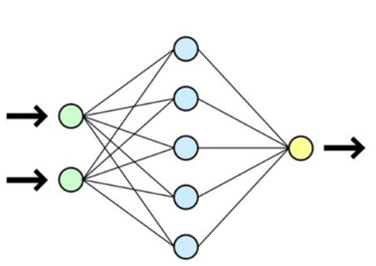
\includegraphics[width=0.7\linewidth]{images/ins}
	\caption{Структура ИНС}
	\label{fig:augexample}
\end{figure}


Типичная структура ИНС (рис. 1) включает:

\begin{itemize}
	\item входной слой, принимающий данные (зелёный цвет);
	\item cкрытые слои, в которых происходит обработка информации (синий цет);
	\item выходной слой, формирующий ответ сети. (желтый цвет).
\end{itemize}


Процесс обучения нейронной сети заключается в подборе весов связей между нейронами таким образом, чтобы минимизировать ошибку между прогнозируемым и фактическим значением. Наиболее распространённым методом оптимизации является обратное распространение ошибки (backpropagation) в сочетании с градиентным спуском.


Нейронные сети бывают различных типов: полносвязные (Dense), сверточные (CNN), рекуррентные (RNN), трансформеры и др. Выбор архитектуры зависит от специфики задачи: для обработки изображений наиболее эффективными зарекомендовали себя сверточные сети, в то время как для анализа последовательностей – рекуррентные и трансформерные модели.

\subsubsection{История и этапы развития нейронных сетей}

Развитие искусственных нейронных сетей прошло несколько ключевых этапов, каждый из которых сопровождался как периодами энтузиазма, так и спадом интереса – так называемыми «зимами искусственного интеллекта».

\begin{enumerate}
	\item Этап зарождения (1940-1960-е гг.):
	
	Первые попытки формализации идей нейронных вычислений относятся к 1943 году, когда Уолтер Питтс и Уоррен МакКаллок представили логико-математическую модель искусственного нейрона. Эта модель, хотя и была простой, заложила фундамент для дальнейших исследований. В 1958 году Фрэнк Розенблатт разработал перцептрон – первую обучаемую нейросеть, способную распознавать простые шаблоны. Однако перцептрон имел ограничения: он не мог решать задачи, в которых классы не разделимы линейно (например, задачи XOR).
	
	\item Первая зима ИИ и застой (1970-1980-е гг.):
	
	После публикации книги Марвина Минского и Сеймура Пейперта Perceptrons (1969), в которой были подробно описаны ограничения перцептрона, интерес к нейросетям значительно снизился. Отсутствие мощных вычислительных ресурсов и недостаток качественных алгоритмов обучения также сыграли свою роль.
	
	\item Возрождения интереса (1986-1990-е гг.):
	
	Ситуация изменилась с появлением алгоритма обратного распространения ошибки (Rumelhart et al., 1986), позволившего эффективно обучать многослойные нейросети. Это открыло путь к построению глубоких моделей. В 1990-е годы нейросети начали использоваться в таких задачах, как распознавание речи, текста и образов.
	
	\item Рождение глубинного обучения (2006-2012 гг.):
	
	Ключевым прорывом стало появление термина «глубинное обучение» (deep learning). Работы Хинтона, Бенжио и Лекуна по автоэнкодерам, сверточным сетям и другим архитектурам позволили строить действительно глубокие модели. В 2012 году модель AlexNet (Крижевский, Хинтон, Суцкевер) выиграла соревнование ImageNet с существенным отрывом, доказав преимущество глубоких сверточных сетей в компьютерном зрении.
	
	\item Современный этап (с 2012 года по настоящее время):
	
	Современные нейросетевые архитектуры (ResNet, EfficientNet, Vision Transformer и др.) достигли впечатляющих результатов в ряде областей – от медицины и автомобильной промышленности до генерации текста и изображений. Развитие специализированных вычислительных платформ (GPU, TPU), доступ к большим данным, а также совершенствование алгоритмов оптимизации сделали обучение сложных моделей доступным и эффективным. Особое внимание уделяется архитектурам с возможностью генерации: GAN, VAE, диффузионные модели и др.
	Таким образом, развитие ИНС представляет собой череду теоретических открытий, технических прорывов и практических применений, которые в совокупности сформировали современный облик машинного обучения.
	
\end{enumerate}

\subsubsection{Современные направления и области применения}

На текущем этапе искусственные нейронные сети (ИНС) стали неотъемлемой частью широкого спектра прикладных и исследовательских задач. Рост вычислительных мощностей, развитие алгоритмов и доступность больших наборов данных способствовали формированию нескольких ключевых направлений применения нейросетевых технологий.

\begin{enumerate}
	\item Обработка изображений и видео.
	
	Сверточные нейронные сети (Convolutional Neural Networks, CNN) обеспечили революцию в компьютерном зрении. Они успешно применяются для:
	
	\begin{itemize}
		\item классификация изображений (ImageNet, CIFAR);
		\item выделения объектов (segmentation);
		\item обнаружения объектов (YOLO, SSD);
		\item распознавания лиц и эмоций;
		\item построения 3D-реконструкций;
		\item восстановления изображений и суперразрешения.
	\end{itemize}
	
	\item Обработка естественного языка (NLP).
	
	Модели трансформерного типа (Transformer, BERT, GPT) позволили достигнуть прорывных результатов в:
	
	\begin{itemize}
		\item машинном переводе;
		\item генерации текста;
		\item извлечении информации;
		\item распознавания лиц и эмоций;
		\item классификации и анализе тональности;
		\item ответах на вопросы и диалоговых системах.
	\end{itemize}
	
	\item Задачи генерации.
	
	Развитие генеративных моделей (в том числе GAN, VAE, Diffusion) дало мощный импульс в таких задачах, как:
	
	\begin{itemize}
		\item генерация фотореалистичных изображений;
		\item стилизация и изменение изображений;
		\item создание видео и 3D-моделей;
		\item распознавания лиц и эмоций;
		\item генерация медицинских снимков для расширения выборок.
	\end{itemize}
	
	\item Медицина.

ИНС используется для анализа рентгеновских снимков, КТ и МРТ, распознавания патологий, поддержки принятия клинических решений. Важное преимущество – способность выявлять паттерны, неочевидные для врача.

	\item Автономный транспорт.
	
Нейросети активно применяются в задачах компьютерного зрения и принятия решений в автономных автомобилях: распознавание дорожных знаков, пешеходов, разметки, прогнозирование траекторий движения.

	\item Финансовый сектор.
	
ИНС используются для прогнозирования временных рядов, обнаружения аномалий (в том числе мошенничества), анализа клиентского поведения и автоматизации поддержки.

	\item Робототехника и промышленность.

Интеллектуальные системы управления, техническое зрение, обработка сигналов с датчиков и предиктивное обслуживание оборудования – все это активно использует нейросети.

	\item Искусство и творчество.

Нейросети генерируют музыку, изображения, видео, стихи и даже сценарии. Развития креативного ИИ расширяет горизонты взаимодействия человека с технологиями.

Таким образом, ИНС охватывают почти все сферы деятельности – от научных исследований до повседневных пользовательских решений. Их универсальность, способность к обучению и высокая точность делают нейросети одним из наиболее перспективных направлений и области ИИ.
	
\end{enumerate}

\subsubsection{Технические ограничения и вызовы при обучении нейронных сетей}

Обучение искусственных нейронных сетей (ИНС) сталкивается с рядом технических ограничений, которые влияют на их эффективность и практическую применимость. Эти вызовы особенно актуальны в условиях ограниченных ресурсов и данных, что делает аугментацию изображений важным инструментом для их преодоления.

\begin{enumerate}
	\item Вычислительные ресурсы:
	
	Современные глубокие нейронные сети требуют значительных вычислительных мощностей, таких как графические процессоры (GPU) или тензорные процессоры (TPU). Отсутствие доступа к таким ресурсам ограничивает масштабируемость моделей, особенно для малого и среднего бизнеса.
	\item Переобучение и недостаток данных: 
	
	При малом объеме обучающих данных ИНС склонны к переобучению, запоминая специфические особенности тренировочной выборки вместо обобщения. Это особенно заметно в задачах с редкими классами или специфическими объектами.
	\item Качество разметки: 
	
	Ошибки в разметке или ее неполнота могут привести к снижению точности модели. Ручная разметка требует значительных затрат времени и ресурсов, особенно в специализированных областях, таких как медицина.
	\item Роль аугментации:
	
	Аугментация изображений позволяет искусственно увеличивать объем данных, улучшать их разнообразие и снижать зависимость от точности разметки. Например, добавление шума или поворотов помогает модели адаптироваться к реальным условиям без необходимости сбора новых данных.
\end{enumerate}

Эти ограничения подчеркивают актуальность разработки программных решений, таких как описываемая в данной работе система аугментации, которая делает обучение ИНС более доступным и эффективным.

\subsubsection{Генеративные нейронные сети}

Генеративные нейронные сети (Generative Neural Networks) представляют собой класс моделей, способных создавать новые дополнительные данные, статистически схожие с исходным обучающим распределением. В контексте обработки изображений эти модели предназначены для генерирования реалистичных изображений, модифицировать существующие, выполнять стилизацию и вносить искажения, полезные для задач аугментации. На рисунке 1.2 представлены базовые афинные преобразования, используемые в аугментации изображения.

\begin{figure}[H]
	\centering
	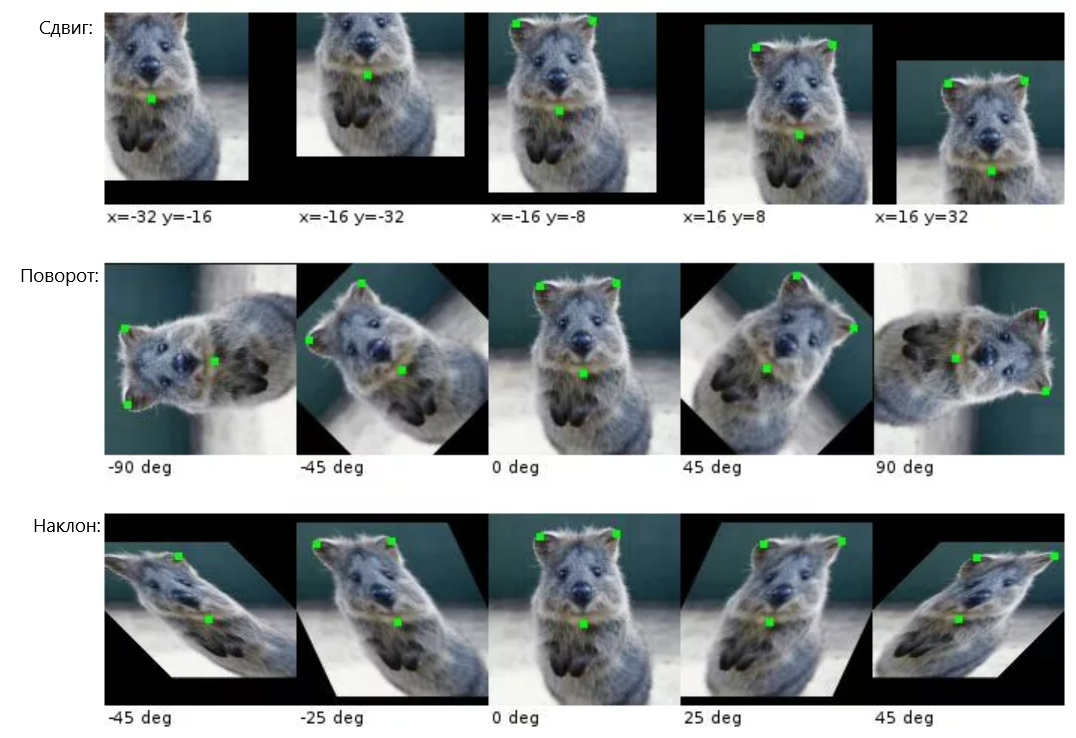
\includegraphics[width=1\linewidth]{images/augexample}
	\caption{Базовые виды аугментации}
	\label{fig:augexample}
\end{figure}


В настоящее время широко используется модель GAN (Generative Neural Networks), которая была предложена Иэном Гудфеллоу в 2014 году. Она состоит из двух нейросетей:

\begin{itemize}
	\item генератор (G) создает изображения на основе случайного шума;
	\item дискриминатор (D) оценивает, являются ли изображения настоящими (из обучающей выборки) или сгенерированными.
\end{itemize}

Обе сети обучаются одновременно при этом генератор стремится обмануть дискриминатор, а дискриминатор – распознать подделку. Такая состязательная структура позволяет достичь высокого качества сгенерированных изображений.

Внедрение в различные области исследований современных технологий привело к разработке разновидностей GAN:
\begin{itemize}
	\item DCGAN – архитектура, основанная на сверточныхнейронных сетях (СНС), применяемая в задачах генерации изображений;
	\item StyleGAN / StyleGAN2 – позволяет управлять стилевыми характеристиками изображения (широко используется в DeepFake, генерации лиц);
	\item CycleGAN – используется для преобразования изображений между двумя доменами без необходимости в парных данных (например, стиль «зима – лето»).
\end{itemize}

Вышеизложенное свидетельствует о том, что технологии GAN находят широкое применение в аугментации объема информации, в тех случаях, когда необходимо увеличить разнообразие изображений сохраняя структуру или стиль.

\textbf{Диффузионные модели}

Одно из наиболее перспективных направлений	 - диффузионные модели (Diffusion Models). В отличие от GAN, они обучаются на задаче поэтапного восстановления изображения из шума.

Процесс включает:

\begin{itemize}
	\item форвард-процесс, где изображение постепенно разрушается путём добавления шума;
	\item реверсивный процесс, где модель обучается восстанавливать изображения обратно шаг за шагом.
\end{itemize}
Примеры моделей:

\begin{itemize}
	\item DDPM (Denoising Diffusion Probabilistic Models) – базовая модель;
	\item Stable Diffusion – открытая и производительная модель для генерации изображений по текстовому описанию;
	\item Imagen / DALLE 2 – модели с высоким качеством генерации, поддерживающие кроссмодальный ввод (текст - изображение).
\end{itemize}

Преимущество применения диффузионных моделей заключается в высокой стабильности и точности при генерации, а также контроле над семантикой изображения. Диффузионные модели активно применяются для синтеза данных в задачах медицинской визуализации и различных технических областях, в которых важно сохранить реалистичность и структурную достоверность. Это свидетельствует о разработке специальных программных средств таких как:

\begin{itemize}
	\item DeepFake – выполняет синтез лиц на основе GAN, используемый как в развлекательной, так и в судебной экспертизе (в том числе для распознавания подделок);
	\item ProGAN / StyleGAN – применяется для генерации лиц высокой реалистичности, включая создание «несуществующих людей»;
	\item CycleGAN для медицины – используется для переноса изображений между различными режимами визуализации (например, МРТ - КТ);
	\item Med-DDPM – диффузионные модели, адаптированные для синтеза медицинских изображений (патологии, опухоли).
\end{itemize}

Таким образом, генеративные нейросети являются мощным инструментом не только в создании новых изображений, но и в аугментации обучающих выборок, особенно в условиях ограниченного объема исходных реальных изображений.

\subsection{Аугментация изображений}
\subsubsection{Понятие аугментации и её цели}

Аугментация изображений (image augmentation) – представляет собой совокупность методов искусственного увеличения обучающей выборки путём модификации исходных изображений без изменения их семантического содержания. Данная технология играет ключевую роль в задачах машинного обучения, связанных с обработкой изображений, поскольку позволяет повысить обобщающую способность моделей, особенно в условиях ограниченных объемов данных.

Основные цели аугментации изображений:

\begin{itemize}
	\item увеличение объема обучающих изображений – позволяет эффективно использовать ограниченный набор исходных изображений, генерируя из них множество вариаций;
	\item снижение переобучения (overfitting) осуществляется за счёт разнообразия входных данных и нейросеть не «запоминает» конкретные изображения, а учится выделять обобщённые признаки;
	\item повышение устойчивости к шумам и искажениям – особенно актуально в реальных условиях, когда изображения могут содержать артефакты, быть смещёнными, плохо освещёнными и т.п.;
	\item имитация реальных условий эксплуатации – например, поворот, масштабирования и сдвиг предназначены для моделирования различных ракурсов и условий съёмки объектов;
	\item балансировка классов в выборке – используется при дисбалансе классов, способствует дополнительнму генерированию изображений в случаях недостаточно представленных категорий;
	\item поддержка робастности – особенно важна в медицинских исследованиях, промышленности и других критичных областях, в которых реализуемые модели должна сохранять точность при отклонениях в данных.
\end{itemize}

Аугментация может применяться как на этапе подготовки данных (оффлайн), так и на динамических этапах во время обучения (онлайн) НС. , Применение этого метода обеспечивает дополнительный объем и разнообразие данных в процессе обучения модели.

Методы аугментации условно делятся на:

\begin{itemize}
	\item классические – основаны на геометрических и цветовых преобразованиях;
	\item генеративные – базируются на нейросетевых моделях, таких как GAN и диффузионные сети.
\end{itemize}

\subsubsection{Методы аугментации изображений}

Классические методы аугментации изображений представляют собой предопределённые трансформации, которые изменяют изображение определённым образом без изменения его смыслового содержания и принадлежности одной генеральной совокупности данных. Эти методы не требуют обучения и широко применяются в промышленности и научных исследованиях благодаря простоте реализации и эффективности.

\paragraph{Геометрические преобразования}

Геометрические преобразования являются одним из наиболее распространённых методов, применяемых в случаях недостаточной информации об анализируемых изображениях со сложной структурой объектов.

Основные афинные преобразования, используемые при изменении положения, ориентации и масштаба объектов на изображении заключаются в следующем:

\begin{itemize}
	\item поворот: изображение поворачивается на случайный или определенный заданный угол, обычно в пределах от -30 до +30 градусов. Это позволяет нейросети быть устойчивой к изменениям угла обзора;
	\item сдвиг пикселей изображения: изображение смещается по горизонтали или вертикали. Сдвиги до 10-20 процентов от размера изображения сохраняют информативность, но создают необходимое разнообразие;
	\item масштабирование: меняется масштаб изображения, как с увеличением, так и с уменьшением. Важно сохранять объект полностью в кадре, чтобы не потерять ключевые признаки;
	\item обрезка: выбирается случайная или центральная часть изображения. Позволяет сделать модель устойчивой к частичному отсутствию информации;
	\item отражение: зеркальное отображение по горизонтали и/или вертикали. Эффективно для симметричных объектов (лица, животные, транспорт);
	\item искажение (Shearing, Affine/Perspective transforms).
\end{itemize}

Геометрические искажения формы объекта, целесообразно применять для моделирования наклонов и перспективных изменений. Геометрические преобразования наиболее эффективных в задачах, где важна пространственная инвариантность – например, в распознавании объектов, медицинской диагностике, анализе сцен.

\paragraph{Цветовые и яркостные искажения}

Изменение цветовых и яркостных искажений предоставляют возможность имититации изменений условий освещения, качества съёмки, особенностей сенсоров и других факторов, влияющих на внешний вид изображения, но не на его семантику. Эти методы повышают устойчивость модели к разнообразным фотометрическим условиям, которые встречаются в реальных данных. Распространенной методикой исследований являются:

\begin{itemize}
	\item изменение яркости: добавление или вычитания значения ко всем пикселям изображения. Позволяет адаптировать модель к условиям пере- или недоэкспонированных снимков;
	\item изменение контрастности: изменение различия между яркими и тёмными участками. Повышает способность модели работать с изображениями разного качества;
	\item изменение насыщенности: управление интенсивностью цвета. При снижении насыщенности изображение приближается к чёрно-белому, что проверяет устойчивость модели к отсутствию цветовой информации;
	\item цветовые преобразования в разных пространствах (HSV, LAB и др.): выполняются преобразования изображения в альтернативные цветовые пространства, где проще и управляемее вносить изменения в яркость, тон и насыщенность;
	\item гамма-коррекция изображений: моделирует особенности различных дисплеев и сенсоров.
\end{itemize}

\paragraph{Шум, искажения, маскирование}

Данная группа методов направлена на повышение устойчивости моделей к частичным повреждениям, шумам и отсутствию информации на изображении. Это особенно актуально для систем, которые функционируют в условиях нестабильного качества входных данных: например, при съёмке на мобильные устройства, в условиях плохой освещённости или при наличии физических повреждений сенсоров.

Для моделирования и отображения подобной информации чаще всего применяют методы:

\begin{enumerate}
	\item Добавление различного вида шумов на изображения таких как:
	\begin{itemize}
	\item гауссов шум: добавление случайных значений, сгенерированных про нормальное распределение, ко всем или части пикселей изображения;
	\item шум «соль и перец»: случайная замена отдельных пикселей на чёрный или белый цвет;
	\item шум Пуассона, спекл-шум и др.: моделируют особенности определённых сенсоров.
	\end{itemize}
	\item Размытие изображений:
	\begin{itemize}
	\item гауссово размытие: мягкое сглаживание изображения, может имитировать расфокус;
	\item размытие в движении: имитация движения камеры или объекта;
	\item медианное: используется для удаления шумов и проверки устойчивости к потере деталей.
	\end{itemize}
	\item Маскирование изображений: случайное зануление или закрашивание фрагментов изображения (например, прямоугольных областей). Это заставляет модель опираться на контекст и не переобучаться на отдельные детали.
	\item JPEG-сжатие: умышленное снижение качества изображения, чтобы повысить устойчивость модели к потерям информации, характерным для изображений в интернете и мессенджерах.
	\item Объединённые методы деградации: комбинация шумов, искажений и потерь качества, имитирующая реальные «грязные» данные – особенно важно при обучении моделей для работы в полевых условиях.
\end{enumerate}

Построенные на основе методов аугментации изображений интеллектуальные системы предназначены для применения в различных областях исследований.

\subsection{Актуальность темы}

Качество и объём обучающей выборки – один из определяющих факторов успеха в обучении нейронных сетей, особенно в задачах компьютерного зрения. Модели глубокого обучения требуют большого количества разнообразных, достоверно размеченных данных, чтобы эффективно обобщать знания и демонстрировать высокую точность на ранее не виденных изображениях.


Недостаточное количество данных, низкое разнообразие, ошибки в разметке или несбалансированность классов могут привести к следующим проблемам:

\begin{itemize}
	\item переобучение (overfitting) – модель запоминает детали тренировочных данных, но плохо обобщает на тестовые;
	\item cнижение точности – особенно на реальных данных, отличающихся от тренировочного распределения;
	\item упущение редких, но значимых признаков – модель не способна корректно распознавать редкие объекты или патологии, если они слабо представлены в выборке.
\end{itemize}

Аугментация изображений решает эти проблемы, расширяя исходную выборку без необходимости сбора новых данных. При грамотной реализации, она: повышает устойчивость модели к шуму и вариативности, имитирует реальные условия съемки, уменьшает зависимость от точной разметки, обеспечивает более равномерное представление классов в выборке.

Таким образом, аугментация – это не просто технический приём, а важный компонент стратегии повышения качества данных, без которого обучение нейронных сетей в большинстве прикладных случаев становится неполноценным.

\subsubsection{Проблемы нехватки и дисбаланса данных}

В реальных задачах компьютерного зрения частого возникает дефицит обучающих данных, особенно если речь идёт о специализированных или чувствительных областях – таких как медицина, безопасность или промышленность. Сбор и разметка изображений в этих сферах могут быть трудоёмкими, дорогостоящими и этически или технически ограниченными. Требуется участие квалифицированных специалистов, лицензирование и соблюдение нормативных требований. Кроме того, в выборках часто наблюдается дисбаланс классов – ситуация, при которой одни категории данных представлены значительно лучше, чем другие. В медицинских изображениях здоровые органы преобладают, а патологии редки. В задачах распознавания объектов на дорогах пешеходов или велосипедистов меньше, чем автомобилей. В промышленных системах дефекты на изделиях представлены в крайне малом объёме. Из-за дисбаланса модель «привыкает» к преобладающим классам и игнорирует редкие, возникает смещения в предсказаниях, ошибки на редких классам могут быть критичны.

Как помогает аугментация:

\begin{itemize}
	\item при нехватке данных: увеличивает объём тренировочной выборки за счёт вариаций исходных изображений;
	\item при дисбалансе: позволяет искусственно дополнить недопредставленные классы;
	\item в условиях конфиденциальности: может применяться на локальных данных без необходимости передачи оригиналов, особенно при генеративных подходах.
\end{itemize}

Таким образом, аугментация становится инструментом не только повышения устойчивости модели, но и устранения фундаментальных ограничений, связанных с доступностью и структурой данных.

\subsubsection{Применение аугментации в прикладных задачах}

Аугментация изображений имеет широкое применение в различных отраслях, где важна точность распознавания визуальных паттернов, но при этом сбор данных затруднён или недостаточен.

\paragraph{Медицина}

В медицинской визуализации аугментация помогает искусственно увеличивать количество изображений с редкими патологиями, повысить устойчивость моделей к различиям в оборудовании (разные контрастность, шумы, разрешение), обучать модели, несмотря на ограничения, связанные с конфиденциальностью и нормативами хранения данных.

Примеры применения:

\begin{itemize}
	\item обнаружение пневмонии на рентгеновских снимках лёгких;
	\item диагностика опухолей на МРТ головного мозга;
	\item cегментация органов на КТ и УЗИ.
\end{itemize}

\paragraph{Автомобильная промышленность}

Автоматизированные системы вождения и системы помощи водителю (ADAS) требуют устойчивости к широкому спектру условий съёмки: дождь, снег, ночь, туман, разные типы камер и т.д.

Примеры применения:

\begin{itemize}
	\item имитация погодных и освещенных условий (яркость, размытие, шум);
	\item cинтетическое дополнение изображения редкими объектами (пешеходами, мотоциклами);
	\item улучшение работы модели при частичном перекрытии объектов (маскирование).
\end{itemize}

\paragraph{Безопасность (распознавание лиц, событий)}

В задачах видеонаблюдения и контроля доступа часто встречаются проблемы низкого качества изображений из-за низкого освещения и шума, частичное перекрытие лиц и объектов, необходимость работы в реальном времени.

Примеры применения:

\begin{itemize}
	\item повышает устойчивость систем к искажениям;
	\item позволяет улучшить обобщающую способность на новых камерах и в разных условиях;
	\item поддерживает задачи распознавания подозрительных действий и событий.
\end{itemize}

\paragraph{Агротехнологии и спутниковый мониторинг}

В сельском хозяйстве и геопространственном анализе используются снимки с дронов и спутников, часто получаемые при разной погоде, высоте и сезоне.


Примеры применения:

\begin{itemize}
	\item создавать дополнительные данные для распознавания болезней растений, вредителей;
	\item обеспечивать устойчивость к разнице в разрешении и масштабе;
	\item использовать модели на снимках из других регионов или сезонов.
\end{itemize}

\subsubsection{Применение аугментации в прикладных задачах}

Переобучение (overfitting) – одна из наиболее распространённых проблем при обучении нейронных сетей, особенно на малых или слабо разнообразных выборках. Модель, столкнувшись с ограниченным числом примеров, «запоминает» данные вместо того, чтобы извлекать обобщающие закономерности. В результате она показывает отличные результаты на тренировочных данных, но значительно теряет точность на новых, ранее не встречавшихся изображениях.

Причины переобучения:

\begin{itemize}
	\item недостаточное количество данных;
	\item однотипные изображения в обучающем наборе;
	\item высокая модельная сложность;
	\item несбалансированные или плохо размеченные классы.
\end{itemize}

Аугментация изображений помогает бороться с переобучением за счёт искусственного увеличения выбора объёма выборки. Каждое оригинальное изображения может быть превращено в десятки универсальных вариантов, что повышает разнообразие данных. Также повышается устойчивость модели: модель обучается «игнорировать» нерелевантные различия, такие как поворот, освещение, масштаб, артефакты съёмки. Создаются ситуации близкие к реальным. Например, генерация изображений с шумом, засветами, низкой резкостью помогает модели справляться с подобными ситуациями на практике. Повышается регуляризация, т.е. аугментация может рассматриваться как форма регуляризации, поскольку она усложняет задачу для модели и вынуждает её искать более устойчивые и обобщённые признаки.

Особенно эффективной считается online-аугментация – когда трансформации применяются к изображениям во время каждой эпохи обучения. Это делает процесс обучения более вариативным и снижает риск запоминания данных.

Таким образом мы можем сказать, что аугментация – это не просто способ увеличения данных, но и важный механизм борьбы с переобучением. Она усиливает обобщающую способность модели, позволяя достигать высокой точности в реальных условиях.
